% !TeX root = ../main.tex
% Add the above to each chapter to make compiling the PDF easier in some editors.

\chapter{Background}\label{chapter:background} % Anshul 4 sayfa yazmış

\section{Cloud Computing Landscape} % Cloud usage scenarios
\subsection{Usage Scenarios}
Cloud computing is becoming increasingly popular as on-demand provisioning capabilities and support for various use cases are growing \cite{cloud-use-cases}. Some of those use cases include file storage like OneDrive, database as a service systems like Amazon SimpleDB, entertainment services such as Netflix, multiplayer online games like Dota 2. Businesses are also using cloud computing for instant messaging between departments through applications like Slack or storing customer data in customer relationship management services provided by companies such as SAP or Salesforce. Many businesses also offload their computing requirements to cloud for data mining or for project management as the Pay-per-use model of cloud is very beneficial for companies because they don't need to maintain a cluster of computers on premise. Cloud computing is also being used to host social networks such as Facebook.com or Twitter.com with their massive monthly user counts, 2.45 billion and 330 million, respectively.

\subsection{Virtualization}
The different use cases explained above are only possible because cloud computing provides abstraction by virtualisation. Real hardware in data centers can be abstracted and be broken to smaller units and can be distributed among customers as virtual machines. This way every customer can have their own personal computer running on the cloud and their system is fully isolated from other customers. While virtual machines were the defacto unit in cloud computing for many years, now there is a new technology called \textit{containerization}. Contaniers allow applications to be packed alongside with their dependencies, and those application can run on the same host OS on top of a container engine. That leads to better utilized servers and less dependency from the underlying hardware. The trade-off is increased delay, because containers add another layer of abstraction on to the stack.

The abstraction in cloud is possible with hypervisor technologies such as Xen. Controlled by software APIs, hypervisors boot self-contained virtual machines on demand, and can run applications as if they were running on physical hosts. This is called \textit{server consolidation} and it has been a great way to reduce under-utilized hardware.

\iffalse
\begin{figure}[htpb]
  \centering
  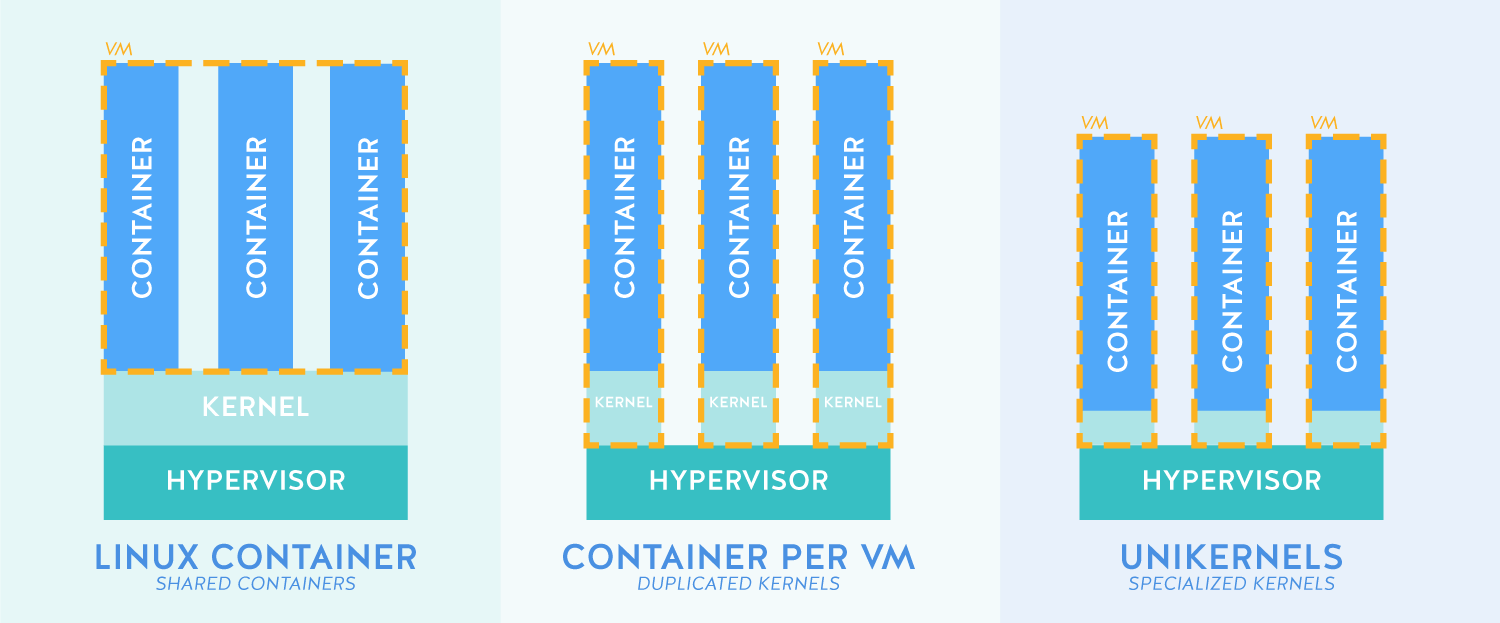
\includegraphics[width=0.4\textwidth]{figures/Linux-containers-vms-unikernels.png}
  \caption{Different virtualization techniques: https://nordicapis.com/introduction-to-unikernels/} \label{fig:virt}
\end{figure}
\fi
\section{Unikernels}
Unikernels \cite{library-operating-system} \cite{madhavapeddy2014unikernels} are specialised machine images compiled from high-level languages. Those machine images can run directly on the hypervisor or on bare metal. First examples of unikernels can be seen since the late 1990's with the projects like Exodus \cite{exokernel} and Nemesis \cite{nemesis}. In a unikernel project, the developer selects libraries from a repository where the OS functionalities are implemented in. In most cases, these libraries are also implemented in the high-level language that the project is implemented. Once the required libraries for the project are selected, whole codebase is compiled with configuration code for the target runtime. The resulting artifact has the modular stack architecture similar to figure \ref{fig:unikernel-arch} and is a single OS image. This OS image can then be distributed analogous to conventional OS images and be booted directly by a hypervisor or installed to hardware through BIOS. They can be uploaded to cloud systems like OpenStack \cite{openstack} to be booted at will or can be distributed to smaller devices, which is the purpose of this project.

\begin{figure}[htpb]
  \centering
  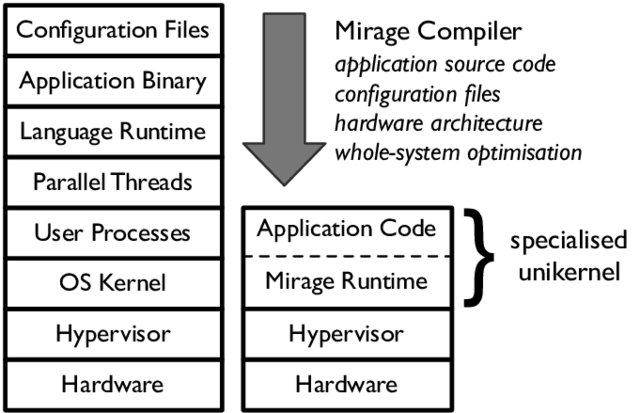
\includegraphics[height=0.3\textwidth]{figures/Contrasting-software-layers-in-existing-VM-appliances-vs-unikernels-standalone-kernel_W640.jpg}
  \caption{ Contrasting software layers in existing VM appliances vs. unikernel’s standalone kernel compilation approach. \cite{library-operating-system}} \label{fig:unikernel-arch}
\end{figure}

Unikernels are currently not production ready \cite{unfit-for-production}. They lack the proper tooling around them and they don't have a "killer-app" for now. However, there is a growing interest around them with startups trying to bring the technology to general usage. One of those startups is Unikernel Systems, based in Cambridge, UK. Unikernel Systems was acquired by Docker in 2016 \cite{docker-acquisiton}. The company consists mostly of developers from the Xen Project. Unikernel technology is more low-level than what Docker provides with its containers and the stated goal of the acqusition is that they want to use the low-level programming expertise of the unikernel team to enchance the power of Docker. All these connections between those three components, namely Docker, Unikernel System and ex-Xen developers show us the big picture of the future cloud techology.

The advantages and drawbacks of using unikernels are explained in the \hyperref[chapter:implementation]{implementation} and \hyperref[chapter:evaluation]{evaluation} part of this thesis with encountered problems and their possible solutions.

The unikernel ecosystem thrives through open source projects. There is currently no production ready unikernel project that can be used for any arbitrary need. There are multiple groups developing unikernel solutions. A small group of these solutions include:
\subsection*{MirageOS}

\url{https://github.com/mirage/mirage} \cite{madhavapeddy2014unikernels}
  MirageOS is a unikernel solution for the OCaml language. It provides libraries for e.g. networking, storage that become operating system drivers when the application is compiled. It produces artifacts that run either on the XEN or KVM hypervisors. It also runs on the ARM64 CPUs, which makes it possible to deploy MirageOS unikernels to Raspberry Pi as IoT targets.
\subsection*{Unik}
\url{https://github.com/solo-io/unik} \cite{levine2016unik} This project brands itself as "Compilation and Deployment Platform" and has support for many providers. It has an API similar to Docker for building unikernels and for managing them. They require a Docker program to be running in the background to manage Unik unikernels properly. They have a wide-range support for different unikernel runtimes such as Osv, MirageOS or Virtualbox. They have a demo of running unikernels on a Kubernetes cluster \cite{unik-youtube}, but there are not instruction to replicate that.
\subsection*{IncludeOS}
\url{https://github.com/includeos/IncludeOS} \cite{7396164}
IncludeOS includes the operating system code to the application as a library when compiled. It can be used to develop C and C++ applications. They target IoT devices as well for improved security. One of their goals is to make IncludeOS bootable on Raspberry Pi M3 B+ models. It supports KVM and some cloud providers such as Google Compute Engine. An IncludeOS image can be booted in tens of milliseconds and only takes 3-4 megabytes in size.

\subsection*{Ops}
\url{https://github.com/nanovms/ops}
  Ops is an interface for creating and managing unikernels in the nanovms infrastructure \cite{nanovms}. It has a wrapper around QEMU \cite{qemu} to run unikernels within the Ops-cli. Ops uses configuration files to embed static content and to configure runtime arguments of images at compile time. It supports multiple languages.
\newline

Some of these projects include Kubernetes as their deployment target but they do it by including a host OS, thus does not use the full potential of unikernels.

There are companies working on development of unikernels. The most prominent one is Docker, which is the defacto standart for containerized applications \cite{francia_2016}. Unikernels were also subject to CNCF conferences in the past.

\section{Orchestration}
The adoption of containers in the IT world is still low but it's growing every year. A survey made by Diamante states that \textit{"in 2018 just 17 percent said that IT operations teams were driving container adoption; a year later that number has jumped to more than 35 percent"} \cite{diamante}. They also state that the reason for this big shift is the improvements in orchestration technology. Currently the most popular orchestration technology is Kubernetes, an open source project, initiated by Google. Kubernetes connects multiple machines together and serves their resources through a single interface for container deployment. It takes the responsibility of running containers from developers and gives it to automation algorithms. It's treating containers as short-lived entities and deploys them again if a container fails or if a better resource utilization oppurtunity is available.

Kubernetes has a communication interface between machines for containers to talk to each other and to outside services. This communication is possible with a Kubernetes daemon called kubelet running on every machine connected to the cluster. This intercluster networking is realised by an internal DNS and load balancers. This networking can be extended by the user with a resource called "Service". With that, different deployments can talk to each other through Kubernetes without requiring an explicit IP address. All low level communication is handled by the Kubernetes stack through a component called "kubeproxy".

Kubernetes' internal load balancer is also useful for scaling. Kubernetes has horizontal scalability functionality for busy containers. If a deployment is taking too much requests, Kubernetes creates replicas of the container, possibly on different machines, thus divides the incoming workload. This is called horizontal scaling and if no custom scaling algorithm is given, handled completely by the cluster. Many cloud providers offer managed Kubernetes clusters as a service, e.g. Google Kubernetes Engine or Amazon Elastic Kubernetes Engine, and if desired, they also increase the number of machines in the cluster if there are no more resources left on the running machines to deploy more replicas. Once those machines become available, Kubernetes' horizontal autoscaling kicks in to utilize those resources.

Kubernetes' popularity comes from the experience of the developers who built it. It's the third generation container-management system developed at Google, a company that has been managing Linux containers for more than ten years \cite{acm-borg}. It grows together with the current trend of microservice architecture, a paradigm that divides bigger applications into smaller units. A kubernetes cluster can support up to 150,000 pods \cite{kubernetes-load}, Kubernetes' smallest unit. It is very customizable and there are many products on top of it in the Cloud Native Computing Foundation to enhance more of its capabilities. Some of those projects in the ecosystem include, e.g. Istio for service meshing, which allows better customisation of inter-cluster communication, Helm for package manager of Kubernetes applications or Envoy as a service proxy.

Kubernetes is the most dominant product on the market right now, but alternatives exists. Some of those alternatives have a more narrowed focus than Kubernetes, providing less capabilities while being easier to operate. A small group of these technologies are as follows:

\subsection*{Docker Swarm}
Docker Swarm is the orchestration solution from the Docker company. It uses the same API as the Docker-cli, so users don't need to learn another set of commands. However, it has less functionality than Kubernetes. For example, secret management of Kubernetes is lacking in Docker Swarm.

\subsection*{Apache Marathon}
Apache Marathon is an orchestrator built on top of Mesos. Mesos is a highly scalable resource manager, also from Apache. Marathon provides scaling, self-healing and service discovery for containerized applications on top of Mesos. It can run both Docker containers and Mesos specific containers.

\subsection*{Hashicorp Nomad}
Nomad follows the *nix philosophy of \textit{"Do One Thing And Do It Well"}. It provides a single binary both for the server and clients, which has a resource manager and a scheduler, while Kubernetes has tens of components to achieve a fully functioning cluster. Nomad also has support for other runtimes such as standalone applications. It can not provide as good customisation as Kubernetes though.

\section{Managing IoT}
It's expected that there will be "20 billion to 35 billion" \cite{unikernels-improve} connected devices in 2020. There are different initiatives to manage this complexity caused by the number of devices out there. Amazon provides device software, connectivity tools and analytics services to their customer to use on their IoT scenarios. Google, like Amazon, provides an IoT Core, a complete pipeline for managing devices and collecting data. While those solutions work, they have a vendor lock-in problem. IoT software is mostly embedded and it's a cumbersome job to move from one software to another one when changing providers. The IoT industry is still a young industry and it lacks unified protocols that are shared by companies providing those services.

A project called K3S \cite{k3s} is a step towards the direction to unify IoT communication. K3S is a Kubernetes distribution aimed for IoT \& edge computing. It supports ARM architecture and can be deployed to a Raspberry Pi device. It can be used to create a connected cluster between a K3S master running in the cloud and IoT devices acting as secondary nodes. K3S uses the same a modified version of the Kubernetes' codebase. The modifications include using \textit{sqlite} as the default storage mechanism instead of \textit{etcd}; packaging required external dependencies with the application; removing cloud provider specific storage plugins. All those modifications aim to provide a single binary for the cluster. Despite using the same codebase, it can't be used together with a normal Kubernetes cluster. That restricts its wide adaption. A company aiming to connect IoT devices through K3S, has to have a K3S deployment on their infrastructure. If they have a Kubernetes cluster for their infrastructure, those clusters can only communicate externally.

Microsoft Azure allows virtual-kubelet, an open source project led by them, to be used with their IoT solutions and with their Kubernetes services \cite{Chandra2019}. A virtual-kubelet instance translates Kubernetes deployment specification to IoT Edge specification, then submits it to the Azure IoT hub. This project "does not provide Kubernetes-backed high availability or disaster recovery to IoT Edge deployments" \cite{azure-vk-github}. Both in Azure's case and in the research proposed by FLEDGE \cite{fledge}, virtual-kubelet was deployed on the cloud and acted as a middle-man between kubernetes and IoT based communication. This thesis deploys virtual-kubelet to IoT devices and cuts the middle-man by providing communication only through Kubernetes.